\documentclass[border=10pt]{standalone}
\usepackage[svgnames]{xcolor}
\usepackage{amsmath}
\usepackage{pgfplots}
\pgfplotsset{compat=newest}
\usepackage[sfdefault]{FiraSans}
\usepackage{FiraMono}
\renewcommand*\familydefault{\sfdefault}
\begin{document}
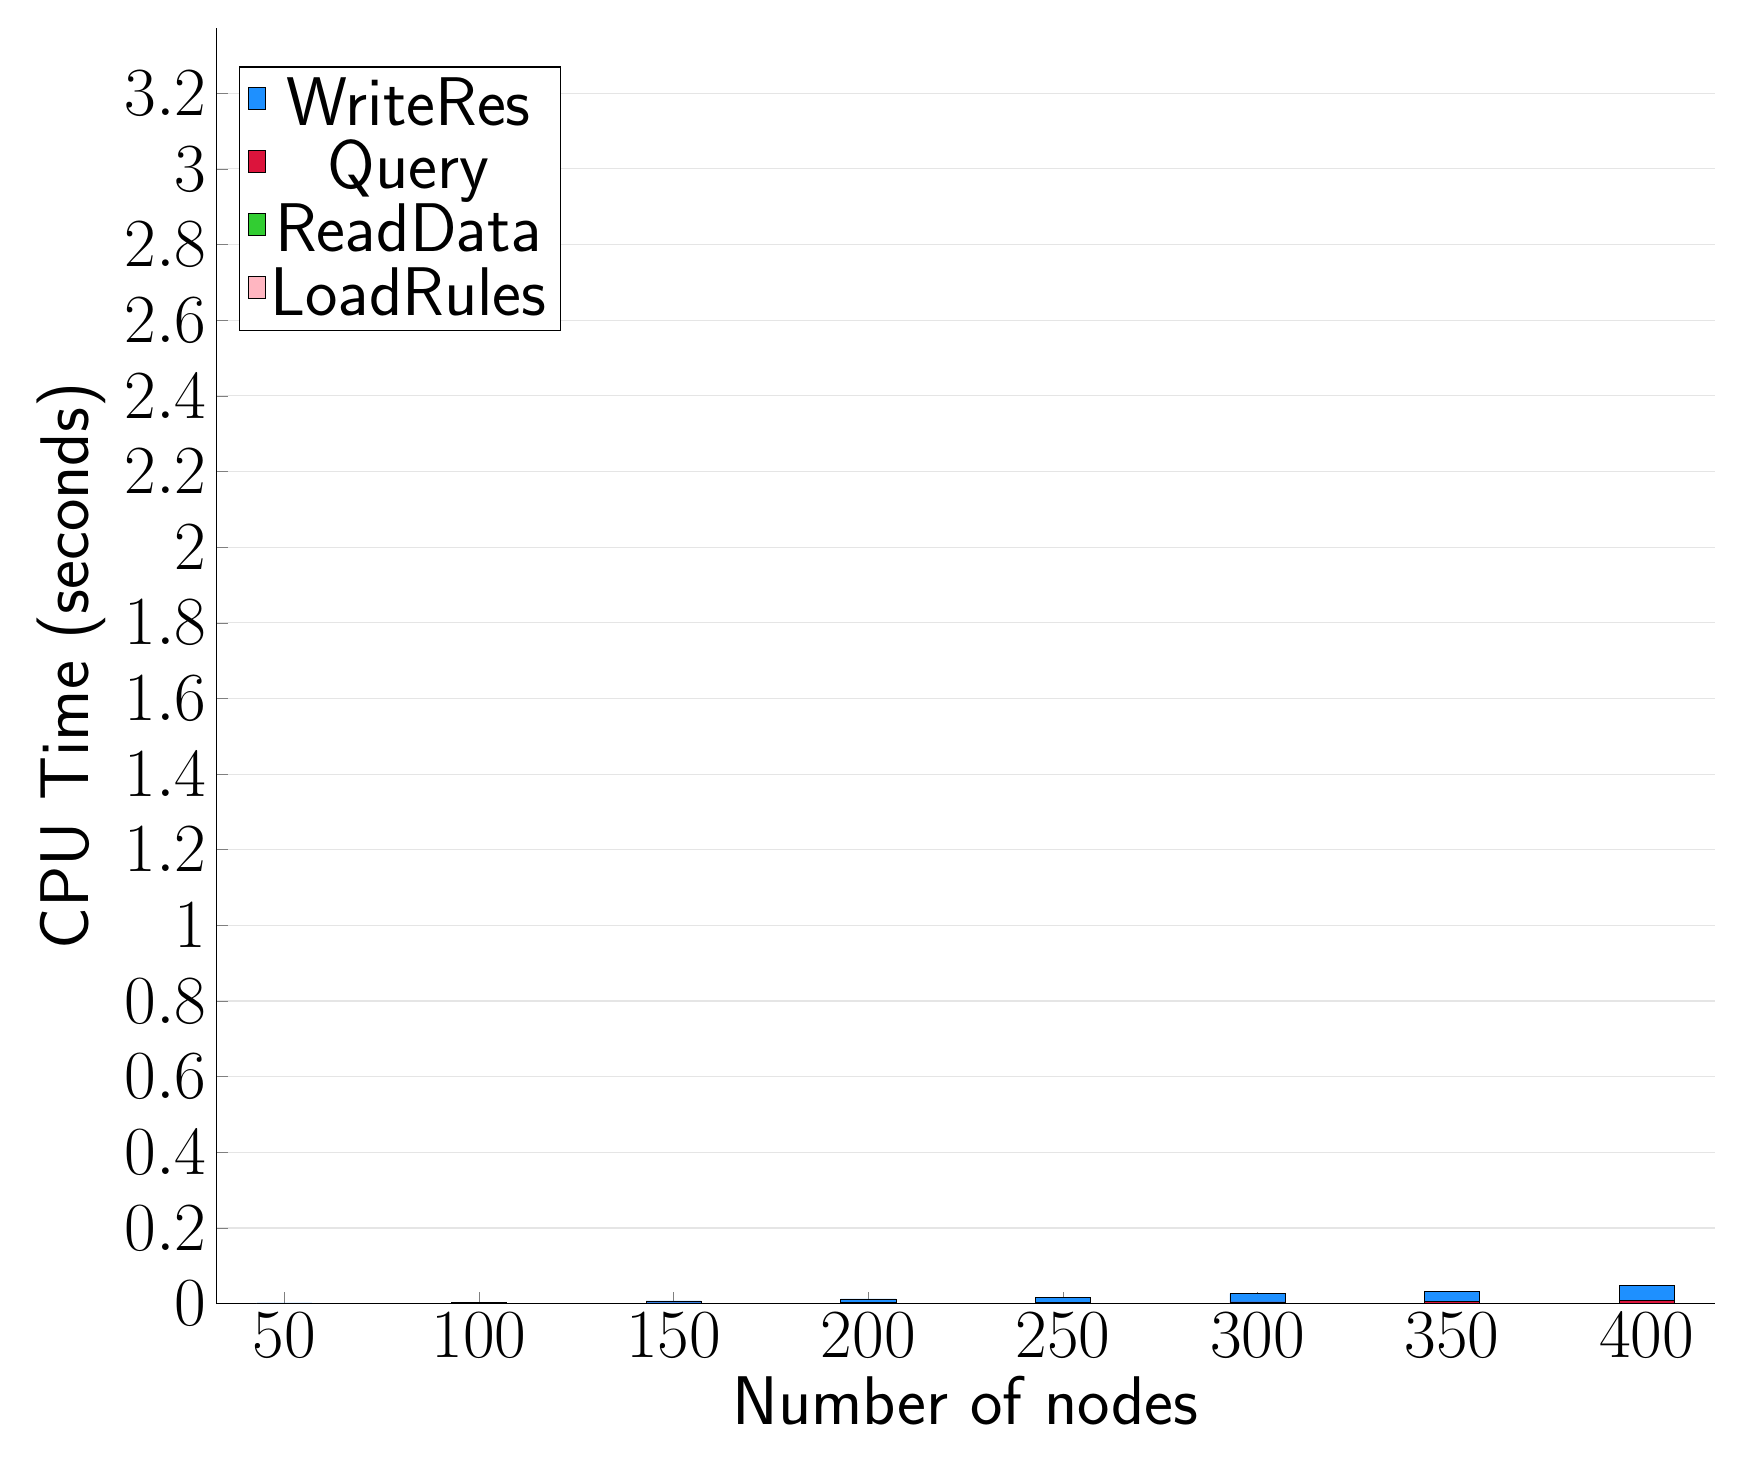
\begin{tikzpicture}
\begin{axis}[
   ybar stacked,
   width=1.7\textwidth,
   bar width=0.7cm,
   ymajorgrids, tick align=inside,
   major grid style={draw=gray!20},
   xtick=data,
   ymin=0, ymax=3.3720000000000003,
   axis x line*=bottom,
   axis y line*=left,
   enlarge x limits=0.05,
   legend style={
       at={(0.23, 0.97)},
       anchor=north east,
       legend columns=1,
       font=\Huge,
   },
   ylabel={CPU Time (seconds)},
   xlabel={Number of nodes},
   label style={font=\Huge},
   tick label style={font=\Huge},
]
\addlegendimage{fill=DodgerBlue, draw=black, line width=0.2pt}
\addlegendentry{WriteRes}
\addlegendimage{fill=Crimson, draw=black, line width=0.2pt}
\addlegendentry{Query}
\addlegendimage{fill=LimeGreen, draw=black, line width=0.2pt}
\addlegendentry{ReadData}
\addlegendimage{fill=LightPink, draw=black, line width=0.2pt}
\addlegendentry{LoadRules}
\addplot +[fill=LightPink, draw=black, line width=0.2pt] coordinates {
(50, 0.0006234)
(100, 0.0006140000000000003)
(150, 0.0005979000000000003)
(200, 0.0006039000000000003)
(250, 0.0006099000000000002)
(300, 0.0006162999999999999)
(350, 0.0006065000000000005)
(400, 0.0006103999999999998)
};
\addplot +[fill=LimeGreen, draw=black, line width=0.2pt] coordinates {
(50, 0.0002159999999999999)
(100, 0.00028549999999999973)
(150, 0.00035489999999999995)
(200, 0.0004419999999999997)
(250, 0.0004924999999999992)
(300, 0.0006106999999999998)
(350, 0.0006636000000000005)
(400, 0.0007914000000000008)
};
\addplot +[fill=Crimson, draw=black, line width=0.2pt] coordinates {
(50, 0.00011319999999999969)
(100, 0.0004071)
(150, 0.0008225000000000003)
(200, 0.0015279)
(250, 0.002016)
(300, 0.0032730000000000003)
(350, 0.0039008000000000003)
(400, 0.0065328999999999995)
};
\addplot +[fill=DodgerBlue, draw=black, line width=0.2pt] coordinates {
(50, 0.0007389999999999999)
(100, 0.0026892)
(150, 0.0055813)
(200, 0.0100794)
(250, 0.013255799999999998)
(300, 0.021685199999999998)
(350, 0.0267913)
(400, 0.0402019)
};
\end{axis}
\end{tikzpicture}

\end{document}
